\documentclass[twoside]{book}

% Packages required by doxygen
\usepackage{fixltx2e}
\usepackage{calc}
\usepackage{doxygen}
\usepackage[export]{adjustbox} % also loads graphicx
\usepackage{graphicx}
\usepackage[utf8]{inputenc}
\usepackage{makeidx}
\usepackage{multicol}
\usepackage{multirow}
\PassOptionsToPackage{warn}{textcomp}
\usepackage{textcomp}
\usepackage[nointegrals]{wasysym}
\usepackage[table]{xcolor}

% Font selection
\usepackage[T1]{fontenc}
\usepackage[scaled=.90]{helvet}
\usepackage{courier}
\usepackage{amssymb}
\usepackage{sectsty}
\renewcommand{\familydefault}{\sfdefault}
\allsectionsfont{%
  \fontseries{bc}\selectfont%
  \color{darkgray}%
}
\renewcommand{\DoxyLabelFont}{%
  \fontseries{bc}\selectfont%
  \color{darkgray}%
}
\newcommand{\+}{\discretionary{\mbox{\scriptsize$\hookleftarrow$}}{}{}}

% Page & text layout
\usepackage{geometry}
\geometry{%
  a4paper,%
  top=2.5cm,%
  bottom=2.5cm,%
  left=2.5cm,%
  right=2.5cm%
}
\tolerance=750
\hfuzz=15pt
\hbadness=750
\setlength{\emergencystretch}{15pt}
\setlength{\parindent}{0cm}
\setlength{\parskip}{3ex plus 2ex minus 2ex}
\makeatletter
\renewcommand{\paragraph}{%
  \@startsection{paragraph}{4}{0ex}{-1.0ex}{1.0ex}{%
    \normalfont\normalsize\bfseries\SS@parafont%
  }%
}
\renewcommand{\subparagraph}{%
  \@startsection{subparagraph}{5}{0ex}{-1.0ex}{1.0ex}{%
    \normalfont\normalsize\bfseries\SS@subparafont%
  }%
}
\makeatother

% Headers & footers
\usepackage{fancyhdr}
\pagestyle{fancyplain}
\fancyhead[LE]{\fancyplain{}{\bfseries\thepage}}
\fancyhead[CE]{\fancyplain{}{}}
\fancyhead[RE]{\fancyplain{}{\bfseries\leftmark}}
\fancyhead[LO]{\fancyplain{}{\bfseries\rightmark}}
\fancyhead[CO]{\fancyplain{}{}}
\fancyhead[RO]{\fancyplain{}{\bfseries\thepage}}
\fancyfoot[LE]{\fancyplain{}{}}
\fancyfoot[CE]{\fancyplain{}{}}
\fancyfoot[RE]{\fancyplain{}{\bfseries\scriptsize Generated by Doxygen }}
\fancyfoot[LO]{\fancyplain{}{\bfseries\scriptsize Generated by Doxygen }}
\fancyfoot[CO]{\fancyplain{}{}}
\fancyfoot[RO]{\fancyplain{}{}}
\renewcommand{\footrulewidth}{0.4pt}
\renewcommand{\chaptermark}[1]{%
  \markboth{#1}{}%
}
\renewcommand{\sectionmark}[1]{%
  \markright{\thesection\ #1}%
}

% Indices & bibliography
\usepackage{natbib}
\usepackage[titles]{tocloft}
\setcounter{tocdepth}{3}
\setcounter{secnumdepth}{5}
\makeindex

% Hyperlinks (required, but should be loaded last)
\usepackage{ifpdf}
\ifpdf
  \usepackage[pdftex,pagebackref=true]{hyperref}
\else
  \usepackage[ps2pdf,pagebackref=true]{hyperref}
\fi
\hypersetup{%
  colorlinks=true,%
  linkcolor=blue,%
  citecolor=blue,%
  unicode%
}

% Custom commands
\newcommand{\clearemptydoublepage}{%
  \newpage{\pagestyle{empty}\cleardoublepage}%
}

\usepackage{caption}
\captionsetup{labelsep=space,justification=centering,font={bf},singlelinecheck=off,skip=4pt,position=top}

%===== C O N T E N T S =====

\begin{document}

% Titlepage & ToC
\hypersetup{pageanchor=false,
             bookmarksnumbered=true,
             pdfencoding=unicode
            }
\pagenumbering{alph}
\begin{titlepage}
\vspace*{7cm}
\begin{center}%
{\Large Maze Robot With Gyro }\\
\vspace*{1cm}
{\large Generated by Doxygen 1.8.13}\\
\end{center}
\end{titlepage}
\clearemptydoublepage
\pagenumbering{roman}
\tableofcontents
\clearemptydoublepage
\pagenumbering{arabic}
\hypersetup{pageanchor=true}

%--- Begin generated contents ---
\chapter{Class Index}
\section{Class List}
Here are the classes, structs, unions and interfaces with brief descriptions\+:\begin{DoxyCompactList}
\item\contentsline{section}{\hyperlink{structCell}{Cell} }{\pageref{structCell}}{}
\item\contentsline{section}{\hyperlink{classIRSensor}{I\+R\+Sensor} \\*Allows for accessing the distance measurements of an IR sensor }{\pageref{classIRSensor}}{}
\item\contentsline{section}{\hyperlink{classMotorDriver}{Motor\+Driver} }{\pageref{classMotorDriver}}{}
\item\contentsline{section}{\hyperlink{classRobot}{Robot} }{\pageref{classRobot}}{}
\end{DoxyCompactList}

\chapter{File Index}
\section{File List}
Here is a list of all documented files with brief descriptions\+:\begin{DoxyCompactList}
\item\contentsline{section}{P\+C\+B\+\_\+test/\+P\+C\+B\+\_\+test/\hyperlink{drive_8h}{drive.\+h} \\*Contains mid-\/level drive commands for the robot, such as driving forward and turning }{\pageref{drive_8h}}{}
\item\contentsline{section}{P\+C\+B\+\_\+test/\+P\+C\+B\+\_\+test/\hyperlink{graph_8h}{graph.\+h} \\*Contains the structure of the maze and functions to alter the robot\textquotesingle{}s relation to the grid }{\pageref{graph_8h}}{}
\item\contentsline{section}{P\+C\+B\+\_\+test/\+P\+C\+B\+\_\+test/\hyperlink{IR_8h}{I\+R.\+h} \\*Contains the \hyperlink{classIRSensor}{I\+R\+Sensor} class, for making IR sensor use easier }{\pageref{IR_8h}}{}
\item\contentsline{section}{P\+C\+B\+\_\+test/\+P\+C\+B\+\_\+test/\hyperlink{PCB__test_8ino}{P\+C\+B\+\_\+test.\+ino} \\*The main file for the project }{\pageref{PCB__test_8ino}}{}
\item\contentsline{section}{P\+C\+B\+\_\+test/\+P\+C\+B\+\_\+test/\hyperlink{TB6612FNG_8h}{T\+B6612\+F\+N\+G.\+h} \\*Contains a low-\/level control interface for the motor driver chip }{\pageref{TB6612FNG_8h}}{}
\item\contentsline{section}{P\+C\+B\+\_\+test/\+P\+C\+B\+\_\+test/\hyperlink{util_8h}{util.\+h} \\*Contains a variety of miscellaneous math functions to allow for cleaner code }{\pageref{util_8h}}{}
\end{DoxyCompactList}

\chapter{Class Documentation}
\hypertarget{structCell}{}\section{Cell Struct Reference}
\label{structCell}\index{Cell@{Cell}}


{\ttfamily \#include $<$graph.\+h$>$}

\subsection*{Public Member Functions}
\begin{DoxyCompactItemize}
\item 
void \hyperlink{structCell_a80aa84cf92ba1b06db0df55f3afbbad3}{add\+Mark} (\hyperlink{util_8h_a92e22a126ad6bf9d255b517e70d083f6}{Direction} d)
\item 
int \hyperlink{structCell_abb4a89d3e0182cf87a3091e0b15d99de}{get\+Mark} (\hyperlink{util_8h_a92e22a126ad6bf9d255b517e70d083f6}{Direction} d)
\end{DoxyCompactItemize}
\subsection*{Public Attributes}
\begin{DoxyCompactItemize}
\item 
\hyperlink{util_8h_a92e22a126ad6bf9d255b517e70d083f6}{Direction} \hyperlink{structCell_a91285699009e9fb89724dc7302d7e9e0}{exits}
\item 
byte \hyperlink{structCell_aba96fc4db8247038613b0bc8be936db9}{marks} \mbox{[}4\mbox{]}
\item 
bool \hyperlink{structCell_aa3a41503f8935cdb70adfb2d35fa7923}{explored}
\end{DoxyCompactItemize}


\subsection{Detailed Description}
The \hyperlink{structCell}{Cell} class represents one grid square of the maze. It stores the cell\textquotesingle{}s available exits, the marks on the cell\textquotesingle{}s edges used by the pathfinding algorithm, and whether or not the cell has been explored or not. Unexplored cells will have every exit marked as blocked (all zeros). 

\subsection{Member Function Documentation}
\mbox{\Hypertarget{structCell_a80aa84cf92ba1b06db0df55f3afbbad3}\label{structCell_a80aa84cf92ba1b06db0df55f3afbbad3}} 
\index{Cell@{Cell}!add\+Mark@{add\+Mark}}
\index{add\+Mark@{add\+Mark}!Cell@{Cell}}
\subsubsection{\texorpdfstring{add\+Mark()}{addMark()}}
{\footnotesize\ttfamily void Cell\+::add\+Mark (\begin{DoxyParamCaption}\item[{\hyperlink{util_8h_a92e22a126ad6bf9d255b517e70d083f6}{Direction}}]{d }\end{DoxyParamCaption})\hspace{0.3cm}{\ttfamily [inline]}}

Adds a mark on the edge of the cell in a given Direction \mbox{\Hypertarget{structCell_abb4a89d3e0182cf87a3091e0b15d99de}\label{structCell_abb4a89d3e0182cf87a3091e0b15d99de}} 
\index{Cell@{Cell}!get\+Mark@{get\+Mark}}
\index{get\+Mark@{get\+Mark}!Cell@{Cell}}
\subsubsection{\texorpdfstring{get\+Mark()}{getMark()}}
{\footnotesize\ttfamily int Cell\+::get\+Mark (\begin{DoxyParamCaption}\item[{\hyperlink{util_8h_a92e22a126ad6bf9d255b517e70d083f6}{Direction}}]{d }\end{DoxyParamCaption})\hspace{0.3cm}{\ttfamily [inline]}}

Returns the number of marks on the edge of the cell in a given Direction 

\subsection{Member Data Documentation}
\mbox{\Hypertarget{structCell_a91285699009e9fb89724dc7302d7e9e0}\label{structCell_a91285699009e9fb89724dc7302d7e9e0}} 
\index{Cell@{Cell}!exits@{exits}}
\index{exits@{exits}!Cell@{Cell}}
\subsubsection{\texorpdfstring{exits}{exits}}
{\footnotesize\ttfamily \hyperlink{util_8h_a92e22a126ad6bf9d255b517e70d083f6}{Direction} Cell\+::exits}

A bitfield representing which exits are open, based on bitwise-\/\+O\+Ring Direction values. When a bit is zero, the corresponding direction is blocked, when one, it is open. \mbox{\Hypertarget{structCell_aa3a41503f8935cdb70adfb2d35fa7923}\label{structCell_aa3a41503f8935cdb70adfb2d35fa7923}} 
\index{Cell@{Cell}!explored@{explored}}
\index{explored@{explored}!Cell@{Cell}}
\subsubsection{\texorpdfstring{explored}{explored}}
{\footnotesize\ttfamily bool Cell\+::explored}

All cells start with explored as \textquotesingle{}false\textquotesingle{}, and are updated to \textquotesingle{}true\textquotesingle{} when the robot has reached it and found the available exits. \mbox{\Hypertarget{structCell_aba96fc4db8247038613b0bc8be936db9}\label{structCell_aba96fc4db8247038613b0bc8be936db9}} 
\index{Cell@{Cell}!marks@{marks}}
\index{marks@{marks}!Cell@{Cell}}
\subsubsection{\texorpdfstring{marks}{marks}}
{\footnotesize\ttfamily byte Cell\+::marks\mbox{[}4\mbox{]}}

Stores the number of marks made on each edge\+: \textquotesingle{}East\textquotesingle{}, \textquotesingle{}North\textquotesingle{}, \textquotesingle{}West\textquotesingle{}, and \textquotesingle{}South\textquotesingle{} respectively. This could be stored in a single byte as the maximum number of marks on a cell is only 2, but the interface is easier to use in array form. 

The documentation for this struct was generated from the following file\+:\begin{DoxyCompactItemize}
\item 
P\+C\+B\+\_\+test/\+P\+C\+B\+\_\+test/\hyperlink{graph_8h}{graph.\+h}\end{DoxyCompactItemize}

\hypertarget{classIRSensor}{}\section{I\+R\+Sensor Class Reference}
\label{classIRSensor}\index{I\+R\+Sensor@{I\+R\+Sensor}}


Allows for accessing the distance measurements of an IR sensor.  




{\ttfamily \#include $<$I\+R.\+h$>$}

\subsection*{Public Member Functions}
\begin{DoxyCompactItemize}
\item 
\mbox{\Hypertarget{classIRSensor_a97ef6ff6b552e5d8e2b378a0a373f463}\label{classIRSensor_a97ef6ff6b552e5d8e2b378a0a373f463}} 
{\bfseries I\+R\+Sensor} (int input\+Pin)
\item 
\mbox{\Hypertarget{classIRSensor_a9567c1b225037c6958b4b20ebff92d81}\label{classIRSensor_a9567c1b225037c6958b4b20ebff92d81}} 
double \hyperlink{classIRSensor_a9567c1b225037c6958b4b20ebff92d81}{get\+Distance} ()
\begin{DoxyCompactList}\small\item\em Returns the current distance in mm. \end{DoxyCompactList}\end{DoxyCompactItemize}


\subsection{Detailed Description}
Allows for accessing the distance measurements of an IR sensor. 

This sensor class averages samples from the IR sensor to get a smooth, consistent measurement of distance, measured in millimeters. 

The documentation for this class was generated from the following file\+:\begin{DoxyCompactItemize}
\item 
P\+C\+B\+\_\+test/\+P\+C\+B\+\_\+test/\hyperlink{IR_8h}{I\+R.\+h}\end{DoxyCompactItemize}

\hypertarget{classMotorDriver}{}\section{Motor\+Driver Class Reference}
\label{classMotorDriver}\index{Motor\+Driver@{Motor\+Driver}}
\subsection*{Public Member Functions}
\begin{DoxyCompactItemize}
\item 
\mbox{\Hypertarget{classMotorDriver_ab763cbf76d38f3357188e483c8cd87bc}\label{classMotorDriver_ab763cbf76d38f3357188e483c8cd87bc}} 
void {\bfseries init} (int reset=-\/1)
\item 
\mbox{\Hypertarget{classMotorDriver_a35a620c31c73aa47b8e76a6552cf670b}\label{classMotorDriver_a35a620c31c73aa47b8e76a6552cf670b}} 
void {\bfseries begin} ()
\item 
\mbox{\Hypertarget{classMotorDriver_a3dd76c4a59d4b77cd2efc132e7a713ce}\label{classMotorDriver_a3dd76c4a59d4b77cd2efc132e7a713ce}} 
void {\bfseries motor\+R\+Forward} (uint8\+\_\+t speed)
\item 
\mbox{\Hypertarget{classMotorDriver_adf9704bce79ad86a155ea626790b1234}\label{classMotorDriver_adf9704bce79ad86a155ea626790b1234}} 
void {\bfseries motor\+L\+Forward} (uint8\+\_\+t speed)
\item 
\mbox{\Hypertarget{classMotorDriver_a8661e41d444ca8ea0e61b30d9473918e}\label{classMotorDriver_a8661e41d444ca8ea0e61b30d9473918e}} 
void {\bfseries motor\+R\+Reverse} (uint8\+\_\+t speed)
\item 
\mbox{\Hypertarget{classMotorDriver_aaba1e81765924194773489637a2e66d6}\label{classMotorDriver_aaba1e81765924194773489637a2e66d6}} 
void {\bfseries motor\+L\+Reverse} (uint8\+\_\+t speed)
\item 
\mbox{\Hypertarget{classMotorDriver_a8c4458f619f1f9148262dcd8b1dcc24a}\label{classMotorDriver_a8c4458f619f1f9148262dcd8b1dcc24a}} 
void {\bfseries motor\+L\+Speed} (int speed)
\item 
\mbox{\Hypertarget{classMotorDriver_ac7127952869669dc12feeb9996220f58}\label{classMotorDriver_ac7127952869669dc12feeb9996220f58}} 
void {\bfseries motor\+R\+Speed} (int speed)
\item 
\mbox{\Hypertarget{classMotorDriver_a3b53531a213492c8755cf77d38d0959a}\label{classMotorDriver_a3b53531a213492c8755cf77d38d0959a}} 
void {\bfseries motor\+Speed} (int l\+Speed, int r\+Speed)
\item 
\mbox{\Hypertarget{classMotorDriver_a4e7f943151af4edb180309445b9df05b}\label{classMotorDriver_a4e7f943151af4edb180309445b9df05b}} 
void {\bfseries stop\+Both\+Motors} ()
\item 
\mbox{\Hypertarget{classMotorDriver_a58a3ff1022bba480555321375bc65696}\label{classMotorDriver_a58a3ff1022bba480555321375bc65696}} 
void {\bfseries stop\+MotorR} ()
\item 
\mbox{\Hypertarget{classMotorDriver_a4703cdb94bfb18b82a5a82f0ec4d5279}\label{classMotorDriver_a4703cdb94bfb18b82a5a82f0ec4d5279}} 
void {\bfseries stop\+MotorL} ()
\end{DoxyCompactItemize}
\subsection*{Protected Attributes}
\begin{DoxyCompactItemize}
\item 
\mbox{\Hypertarget{classMotorDriver_a1c00b6e8c8f56d316f20cf6f12cb9de2}\label{classMotorDriver_a1c00b6e8c8f56d316f20cf6f12cb9de2}} 
int {\bfseries pwm\+R\+\_\+pin}
\item 
\mbox{\Hypertarget{classMotorDriver_a9302f271eff09cfedd12e16720de1824}\label{classMotorDriver_a9302f271eff09cfedd12e16720de1824}} 
int {\bfseries pwm\+L\+\_\+pin}
\item 
\mbox{\Hypertarget{classMotorDriver_a286e7cb87f9bca34e18966cc12d0a81b}\label{classMotorDriver_a286e7cb87f9bca34e18966cc12d0a81b}} 
int {\bfseries Rdir\+\_\+pin}
\item 
\mbox{\Hypertarget{classMotorDriver_ad250a07d6eaf7bd79558c0ef7a7876e8}\label{classMotorDriver_ad250a07d6eaf7bd79558c0ef7a7876e8}} 
int {\bfseries Ldir\+\_\+pin}
\item 
\mbox{\Hypertarget{classMotorDriver_a07c7a59a2eb80a2b489fc61145a34bb9}\label{classMotorDriver_a07c7a59a2eb80a2b489fc61145a34bb9}} 
int {\bfseries reset\+\_\+pin}
\end{DoxyCompactItemize}


The documentation for this class was generated from the following file\+:\begin{DoxyCompactItemize}
\item 
P\+C\+B\+\_\+test/\+P\+C\+B\+\_\+test/\hyperlink{TB6612FNG_8h}{T\+B6612\+F\+N\+G.\+h}\end{DoxyCompactItemize}

\hypertarget{classRobot}{}\section{Robot Class Reference}
\label{classRobot}\index{Robot@{Robot}}


{\ttfamily \#include $<$drive.\+h$>$}

\subsection*{Public Member Functions}
\begin{DoxyCompactItemize}
\item 
\mbox{\Hypertarget{classRobot_a990e86a39cb249629a0985e71211fa2e}\label{classRobot_a990e86a39cb249629a0985e71211fa2e}} 
void {\bfseries init} ()
\item 
\mbox{\Hypertarget{classRobot_a5b1079b77286f963c509b5faa6eb086e}\label{classRobot_a5b1079b77286f963c509b5faa6eb086e}} 
void {\bfseries all\+Stop} ()
\item 
\mbox{\Hypertarget{classRobot_ae98f6f49a4cbe9a2d3741d22483dea65}\label{classRobot_ae98f6f49a4cbe9a2d3741d22483dea65}} 
void {\bfseries turn\+Left} (int spd)
\item 
\mbox{\Hypertarget{classRobot_ab9641c762bcded8d42b44d54b4a88796}\label{classRobot_ab9641c762bcded8d42b44d54b4a88796}} 
void {\bfseries turn\+Right} (int spd)
\item 
\mbox{\Hypertarget{classRobot_a592f08d965facad4153cc6dafc0dc2c5}\label{classRobot_a592f08d965facad4153cc6dafc0dc2c5}} 
void {\bfseries forward} (int spd)
\item 
\mbox{\Hypertarget{classRobot_a620dfa100c49bdcc9adea47f74c88a43}\label{classRobot_a620dfa100c49bdcc9adea47f74c88a43}} 
void {\bfseries reverse} (int spd)
\item 
\mbox{\Hypertarget{classRobot_a872c305b49b0733696a5348e2c8e41c7}\label{classRobot_a872c305b49b0733696a5348e2c8e41c7}} 
void {\bfseries drive} (int l\+Spd, int r\+Spd)
\item 
void \hyperlink{classRobot_a88211ed70c106b8b0c1c0edec49c87a4}{drive\+P\+ID} (double l\+Spd, double r\+Spd)
\begin{DoxyCompactList}\small\item\em Uses P\+ID control to drive the robot at a certain speed. \end{DoxyCompactList}\item 
long \hyperlink{classRobot_ab85e483abd6bb9eb1a3822b44f66aa35}{read\+L\+Enc} ()
\item 
long \hyperlink{classRobot_a2bc5b4f70b378e51c9bef971d24c3465}{read\+R\+Enc} ()
\item 
void \hyperlink{classRobot_a16a8fc6dbaa682231fc5f02754d3d686}{turn\+Angle} (double angle)
\item 
void \hyperlink{classRobot_a7f156346f70997f29e326d0d96acc4d0}{update\+P\+ID} ()
\end{DoxyCompactItemize}


\subsection{Detailed Description}
The \hyperlink{classRobot}{Robot} class provides functions to drive the D\+F\+E\+C\+Bot. 

\subsection{Member Function Documentation}
\mbox{\Hypertarget{classRobot_a88211ed70c106b8b0c1c0edec49c87a4}\label{classRobot_a88211ed70c106b8b0c1c0edec49c87a4}} 
\index{Robot@{Robot}!drive\+P\+ID@{drive\+P\+ID}}
\index{drive\+P\+ID@{drive\+P\+ID}!Robot@{Robot}}
\subsubsection{\texorpdfstring{drive\+P\+I\+D()}{drivePID()}}
{\footnotesize\ttfamily void Robot\+::drive\+P\+ID (\begin{DoxyParamCaption}\item[{double}]{l\+Spd,  }\item[{double}]{r\+Spd }\end{DoxyParamCaption})\hspace{0.3cm}{\ttfamily [inline]}}



Uses P\+ID control to drive the robot at a certain speed. 

Note that speed inputs to this function are in the range \mbox{[}-\/1.\+0, 1.\+0\mbox{]}. This function does not block. \mbox{\Hypertarget{classRobot_ab85e483abd6bb9eb1a3822b44f66aa35}\label{classRobot_ab85e483abd6bb9eb1a3822b44f66aa35}} 
\index{Robot@{Robot}!read\+L\+Enc@{read\+L\+Enc}}
\index{read\+L\+Enc@{read\+L\+Enc}!Robot@{Robot}}
\subsubsection{\texorpdfstring{read\+L\+Enc()}{readLEnc()}}
{\footnotesize\ttfamily long Robot\+::read\+L\+Enc (\begin{DoxyParamCaption}{ }\end{DoxyParamCaption})\hspace{0.3cm}{\ttfamily [inline]}}

Returns the current raw value of the left encoder (in E\+D\+G\+ES) \mbox{\Hypertarget{classRobot_a2bc5b4f70b378e51c9bef971d24c3465}\label{classRobot_a2bc5b4f70b378e51c9bef971d24c3465}} 
\index{Robot@{Robot}!read\+R\+Enc@{read\+R\+Enc}}
\index{read\+R\+Enc@{read\+R\+Enc}!Robot@{Robot}}
\subsubsection{\texorpdfstring{read\+R\+Enc()}{readREnc()}}
{\footnotesize\ttfamily long Robot\+::read\+R\+Enc (\begin{DoxyParamCaption}{ }\end{DoxyParamCaption})\hspace{0.3cm}{\ttfamily [inline]}}

Returns the current raw value of the right encoder (in E\+D\+G\+ES) \mbox{\Hypertarget{classRobot_a16a8fc6dbaa682231fc5f02754d3d686}\label{classRobot_a16a8fc6dbaa682231fc5f02754d3d686}} 
\index{Robot@{Robot}!turn\+Angle@{turn\+Angle}}
\index{turn\+Angle@{turn\+Angle}!Robot@{Robot}}
\subsubsection{\texorpdfstring{turn\+Angle()}{turnAngle()}}
{\footnotesize\ttfamily void Robot\+::turn\+Angle (\begin{DoxyParamCaption}\item[{double}]{angle }\end{DoxyParamCaption})\hspace{0.3cm}{\ttfamily [inline]}}

Turns the robot a specified number of degrees. Positive means counterclockwise, as viewed from above the robot. This function blocks. \mbox{\Hypertarget{classRobot_a7f156346f70997f29e326d0d96acc4d0}\label{classRobot_a7f156346f70997f29e326d0d96acc4d0}} 
\index{Robot@{Robot}!update\+P\+ID@{update\+P\+ID}}
\index{update\+P\+ID@{update\+P\+ID}!Robot@{Robot}}
\subsubsection{\texorpdfstring{update\+P\+I\+D()}{updatePID()}}
{\footnotesize\ttfamily void Robot\+::update\+P\+ID (\begin{DoxyParamCaption}{ }\end{DoxyParamCaption})\hspace{0.3cm}{\ttfamily [inline]}}

Recalculates the motor output power based on the current setpoints--note that this does N\+OT actually set the motors to the new speed! 

The documentation for this class was generated from the following file\+:\begin{DoxyCompactItemize}
\item 
P\+C\+B\+\_\+test/\+P\+C\+B\+\_\+test/\hyperlink{drive_8h}{drive.\+h}\end{DoxyCompactItemize}

\chapter{File Documentation}
\hypertarget{drive_8h}{}\section{P\+C\+B\+\_\+test/\+P\+C\+B\+\_\+test/drive.h File Reference}
\label{drive_8h}\index{P\+C\+B\+\_\+test/\+P\+C\+B\+\_\+test/drive.\+h@{P\+C\+B\+\_\+test/\+P\+C\+B\+\_\+test/drive.\+h}}


Contains mid-\/level drive commands for the robot, such as driving forward and turning.  


{\ttfamily \#include \char`\"{}T\+B6612\+F\+N\+G.\+h\char`\"{}}\newline
{\ttfamily \#include $<$Encoder.\+h$>$}\newline
{\ttfamily \#include \char`\"{}util.\+h\char`\"{}}\newline
Include dependency graph for drive.\+h\+:
\nopagebreak
\begin{figure}[H]
\begin{center}
\leavevmode
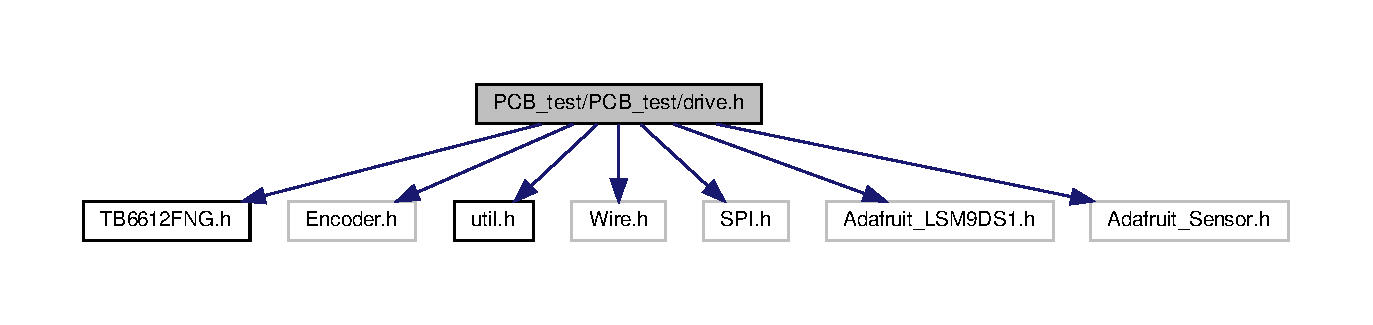
\includegraphics[width=296pt]{drive_8h__incl}
\end{center}
\end{figure}
This graph shows which files directly or indirectly include this file\+:
\nopagebreak
\begin{figure}[H]
\begin{center}
\leavevmode
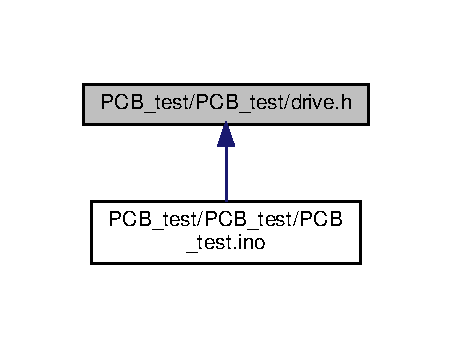
\includegraphics[width=217pt]{drive_8h__dep__incl}
\end{center}
\end{figure}
\subsection*{Classes}
\begin{DoxyCompactItemize}
\item 
class \hyperlink{classRobot}{Robot}
\end{DoxyCompactItemize}
\subsection*{Functions}
\begin{DoxyCompactItemize}
\item 
\mbox{\Hypertarget{drive_8h_a83d1a5e8551e4f9461bc5beb6026fdd8}\label{drive_8h_a83d1a5e8551e4f9461bc5beb6026fdd8}} 
double {\bfseries degrees\+To\+Edges} (double deg)
\end{DoxyCompactItemize}
\subsection*{Variables}
\begin{DoxyCompactItemize}
\item 
\mbox{\Hypertarget{drive_8h_a9b48e465bd56bdf84200e8ca183976db}\label{drive_8h_a9b48e465bd56bdf84200e8ca183976db}} 
constexpr const double {\bfseries edges\+\_\+per\+\_\+mm} = 9.\+4024 $\ast$ 0.\+813
\end{DoxyCompactItemize}


\subsection{Detailed Description}
Contains mid-\/level drive commands for the robot, such as driving forward and turning. 


\hypertarget{graph_8h}{}\section{P\+C\+B\+\_\+test/\+P\+C\+B\+\_\+test/graph.h File Reference}
\label{graph_8h}\index{P\+C\+B\+\_\+test/\+P\+C\+B\+\_\+test/graph.\+h@{P\+C\+B\+\_\+test/\+P\+C\+B\+\_\+test/graph.\+h}}


Contains the structure of the maze and functions to alter the robot\textquotesingle{}s relation to the grid.  


{\ttfamily \#include \char`\"{}util.\+h\char`\"{}}\newline
Include dependency graph for graph.\+h\+:
\nopagebreak
\begin{figure}[H]
\begin{center}
\leavevmode
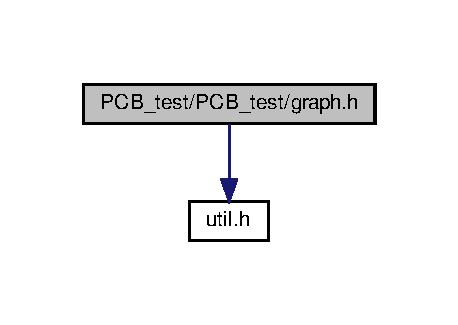
\includegraphics[width=220pt]{graph_8h__incl}
\end{center}
\end{figure}
This graph shows which files directly or indirectly include this file\+:
\nopagebreak
\begin{figure}[H]
\begin{center}
\leavevmode
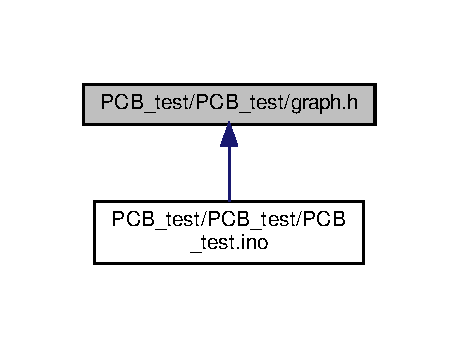
\includegraphics[width=220pt]{graph_8h__dep__incl}
\end{center}
\end{figure}
\subsection*{Classes}
\begin{DoxyCompactItemize}
\item 
struct \hyperlink{structCell}{Cell}
\end{DoxyCompactItemize}
\subsection*{Functions}
\begin{DoxyCompactItemize}
\item 
\mbox{\Hypertarget{graph_8h_a70bc642a7c7b9b1a4752cf04d689e5ec}\label{graph_8h_a70bc642a7c7b9b1a4752cf04d689e5ec}} 
void {\bfseries move\+In} (\hyperlink{util_8h_a92e22a126ad6bf9d255b517e70d083f6}{Direction} dir)
\item 
\hyperlink{util_8h_a92e22a126ad6bf9d255b517e70d083f6}{Direction} \hyperlink{graph_8h_ab4afdc4009e71e9811133449a48262c6}{get\+Relative\+Heading} (int offset)
\end{DoxyCompactItemize}
\subsection*{Variables}
\begin{DoxyCompactItemize}
\item 
\mbox{\Hypertarget{graph_8h_af1b7aa56fe5bbc2c1965c92ea3c6b1a4}\label{graph_8h_af1b7aa56fe5bbc2c1965c92ea3c6b1a4}} 
constexpr const float {\bfseries wall\+\_\+thickness} = 12.\+0
\item 
\mbox{\Hypertarget{graph_8h_ae09ec5e6a6fc4579aec5c96e98ab72da}\label{graph_8h_ae09ec5e6a6fc4579aec5c96e98ab72da}} 
constexpr const float {\bfseries cell\+\_\+width} = 167.\+0 + wall\+\_\+thickness
\item 
\mbox{\Hypertarget{graph_8h_aa2936ecd84787e1d190c651258baaf61}\label{graph_8h_aa2936ecd84787e1d190c651258baaf61}} 
\hyperlink{structCell}{Cell} {\bfseries maze} \mbox{[}10\mbox{]}\mbox{[}10\mbox{]} = \{ \hyperlink{structCell}{Cell}\{ 0, \{ 0 \}, false \} \}
\item 
\mbox{\Hypertarget{graph_8h_af1d3cff2e4538e23400e260bae3dadad}\label{graph_8h_af1d3cff2e4538e23400e260bae3dadad}} 
int {\bfseries row} = 0
\item 
\mbox{\Hypertarget{graph_8h_afb52e720f5f0c483db5861f9e42e924e}\label{graph_8h_afb52e720f5f0c483db5861f9e42e924e}} 
int {\bfseries col} = 0
\item 
\mbox{\Hypertarget{graph_8h_a58d94fa8f7ddf189cd6eabdea4f2346c}\label{graph_8h_a58d94fa8f7ddf189cd6eabdea4f2346c}} 
\hyperlink{util_8h_a92e22a126ad6bf9d255b517e70d083f6}{Direction} {\bfseries dir} = Direction\+::\+East
\end{DoxyCompactItemize}


\subsection{Detailed Description}
Contains the structure of the maze and functions to alter the robot\textquotesingle{}s relation to the grid. 



\subsection{Function Documentation}
\mbox{\Hypertarget{graph_8h_ab4afdc4009e71e9811133449a48262c6}\label{graph_8h_ab4afdc4009e71e9811133449a48262c6}} 
\index{graph.\+h@{graph.\+h}!get\+Relative\+Heading@{get\+Relative\+Heading}}
\index{get\+Relative\+Heading@{get\+Relative\+Heading}!graph.\+h@{graph.\+h}}
\subsubsection{\texorpdfstring{get\+Relative\+Heading()}{getRelativeHeading()}}
{\footnotesize\ttfamily \hyperlink{util_8h_a92e22a126ad6bf9d255b517e70d083f6}{Direction} get\+Relative\+Heading (\begin{DoxyParamCaption}\item[{int}]{offset }\end{DoxyParamCaption})}

This gets the cardinal direction relative to the robot\textquotesingle{}s current heading offset = 0 =$>$ the direction the robot is facing offset = 1 =$>$ the direction to the robot\textquotesingle{}s left offset = -\/1 =$>$ the direction to the robot\textquotesingle{}s right offset = 2 =$>$ the direction behind the robot etc. 
\hypertarget{IR_8h}{}\section{P\+C\+B\+\_\+test/\+P\+C\+B\+\_\+test/\+IR.h File Reference}
\label{IR_8h}\index{P\+C\+B\+\_\+test/\+P\+C\+B\+\_\+test/\+I\+R.\+h@{P\+C\+B\+\_\+test/\+P\+C\+B\+\_\+test/\+I\+R.\+h}}


Contains the \hyperlink{classIRSensor}{I\+R\+Sensor} class, for making IR sensor use easier.  


This graph shows which files directly or indirectly include this file\+:
\nopagebreak
\begin{figure}[H]
\begin{center}
\leavevmode
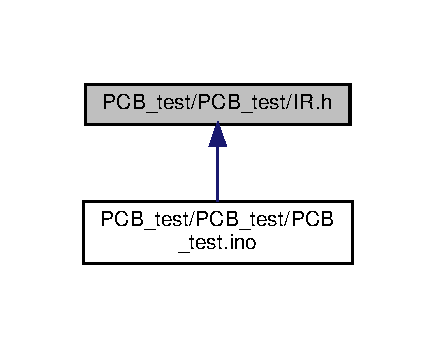
\includegraphics[width=209pt]{IR_8h__dep__incl}
\end{center}
\end{figure}
\subsection*{Classes}
\begin{DoxyCompactItemize}
\item 
class \hyperlink{classIRSensor}{I\+R\+Sensor}
\begin{DoxyCompactList}\small\item\em Allows for accessing the distance measurements of an IR sensor. \end{DoxyCompactList}\end{DoxyCompactItemize}
\subsection*{Variables}
\begin{DoxyCompactItemize}
\item 
\mbox{\Hypertarget{IR_8h_a58a08a86c9319aacf2a6f4f384a9a6a7}\label{IR_8h_a58a08a86c9319aacf2a6f4f384a9a6a7}} 
constexpr const size\+\_\+t {\bfseries I\+R\+\_\+samples} = 100
\end{DoxyCompactItemize}


\subsection{Detailed Description}
Contains the \hyperlink{classIRSensor}{I\+R\+Sensor} class, for making IR sensor use easier. 


\hypertarget{PCB__test_8ino}{}\section{P\+C\+B\+\_\+test/\+P\+C\+B\+\_\+test/\+P\+C\+B\+\_\+test.ino File Reference}
\label{PCB__test_8ino}\index{P\+C\+B\+\_\+test/\+P\+C\+B\+\_\+test/\+P\+C\+B\+\_\+test.\+ino@{P\+C\+B\+\_\+test/\+P\+C\+B\+\_\+test/\+P\+C\+B\+\_\+test.\+ino}}


The main file for the project.  


{\ttfamily \#include \char`\"{}T\+B6612\+F\+N\+G.\+h\char`\"{}}\newline
{\ttfamily \#include \char`\"{}drive.\+h\char`\"{}}\newline
{\ttfamily \#include \char`\"{}I\+R.\+h\char`\"{}}\newline
{\ttfamily \#include \char`\"{}graph.\+h\char`\"{}}\newline
Include dependency graph for P\+C\+B\+\_\+test.\+ino\+:\nopagebreak
\begin{figure}[H]
\begin{center}
\leavevmode
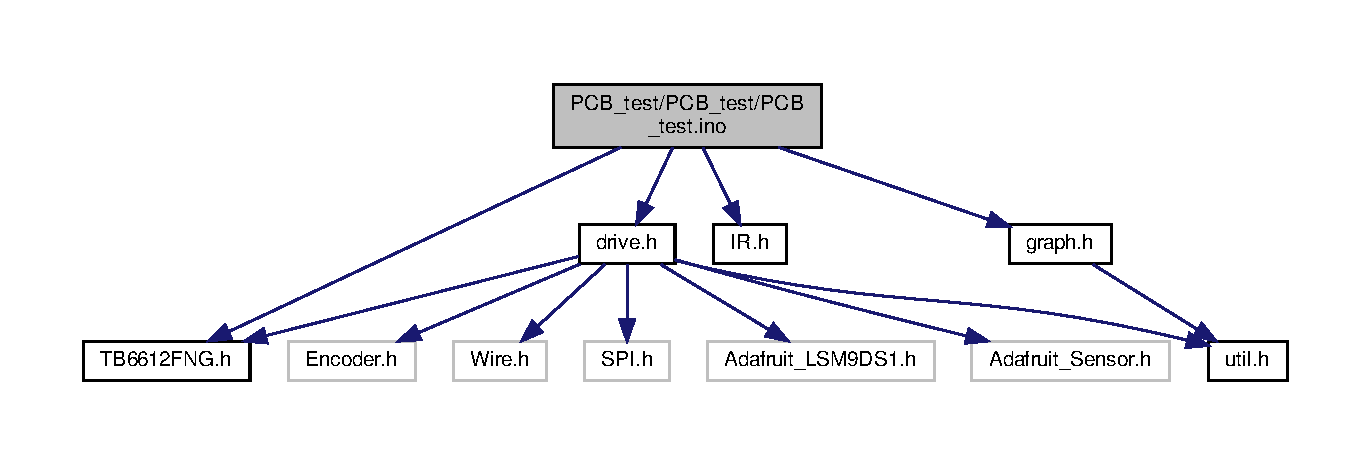
\includegraphics[width=350pt]{PCB__test_8ino__incl}
\end{center}
\end{figure}
\subsection*{Functions}
\begin{DoxyCompactItemize}
\item 
\mbox{\Hypertarget{PCB__test_8ino_ab7aece27431c153f5407864297b7c32b}\label{PCB__test_8ino_ab7aece27431c153f5407864297b7c32b}} 
void {\bfseries drive\+I\+R\+Adjust} (double spd)
\item 
\mbox{\Hypertarget{PCB__test_8ino_a56dfd95fece10fad4869ceb37cfe035d}\label{PCB__test_8ino_a56dfd95fece10fad4869ceb37cfe035d}} 
void {\bfseries drive\+Distance} (double mm)
\item 
\mbox{\Hypertarget{PCB__test_8ino_abe60ad2fecd7fb38997addbd92d88c68}\label{PCB__test_8ino_abe60ad2fecd7fb38997addbd92d88c68}} 
\hyperlink{util_8h_a92e22a126ad6bf9d255b517e70d083f6}{Direction} \hyperlink{PCB__test_8ino_abe60ad2fecd7fb38997addbd92d88c68}{next\+Move} ()
\begin{DoxyCompactList}\small\item\em Determines the next direction to be traveled in based on th Trémaux algorithm. s. \end{DoxyCompactList}\item 
\hyperlink{util_8h_a92e22a126ad6bf9d255b517e70d083f6}{Direction} \hyperlink{PCB__test_8ino_abc9fd4d649a1719e3e8f25cf3fd22857}{explore\+Edge} (long l\+Start, long r\+Start, bool need\+Acceleration)
\begin{DoxyCompactList}\small\item\em Moves the robot into the next cell, updates the cell, and readies the robot for its next action. \end{DoxyCompactList}\item 
\mbox{\Hypertarget{PCB__test_8ino_ad9d79fb25b7ad31450ea631b61f1883e}\label{PCB__test_8ino_ad9d79fb25b7ad31450ea631b61f1883e}} 
void \hyperlink{PCB__test_8ino_ad9d79fb25b7ad31450ea631b61f1883e}{wait\+For\+Power} ()
\begin{DoxyCompactList}\small\item\em Stops the robot\textquotesingle{}s movement and waits for the motor driver to be powered. \end{DoxyCompactList}\item 
\mbox{\Hypertarget{PCB__test_8ino_a25f18de883c5d893238db0b25fb9f471}\label{PCB__test_8ino_a25f18de883c5d893238db0b25fb9f471}} 
void {\bfseries update\+Cell} ()
\item 
\mbox{\Hypertarget{PCB__test_8ino_a4fc01d736fe50cf5b977f755b675f11d}\label{PCB__test_8ino_a4fc01d736fe50cf5b977f755b675f11d}} 
void {\bfseries setup} ()
\item 
int \hyperlink{PCB__test_8ino_a1f32d7057151c1c7f0f16a945a27af1e}{count\+Consecutive\+Turns} (\hyperlink{util_8h_a92e22a126ad6bf9d255b517e70d083f6}{Direction} next\+Dir)
\item 
\mbox{\Hypertarget{PCB__test_8ino_afe461d27b9c48d5921c00d521181f12f}\label{PCB__test_8ino_afe461d27b9c48d5921c00d521181f12f}} 
void {\bfseries loop} ()
\end{DoxyCompactItemize}
\subsection*{Variables}
\begin{DoxyCompactItemize}
\item 
\mbox{\Hypertarget{PCB__test_8ino_a1e70493ed842f246d8063b125681035b}\label{PCB__test_8ino_a1e70493ed842f246d8063b125681035b}} 
const double {\bfseries base\+\_\+speed} = 0.\+1
\item 
\mbox{\Hypertarget{PCB__test_8ino_ae30d704126646e0796e7ae5bf81cf672}\label{PCB__test_8ino_ae30d704126646e0796e7ae5bf81cf672}} 
const double {\bfseries bonus\+\_\+speed} = 0.\+25
\item 
\mbox{\Hypertarget{PCB__test_8ino_a3890cece9117b131b8bcb75369f4dfee}\label{PCB__test_8ino_a3890cece9117b131b8bcb75369f4dfee}} 
bool {\bfseries returning} = false
\item 
\mbox{\Hypertarget{PCB__test_8ino_a212e6b8f7e9ed2662711ad228dfc3e25}\label{PCB__test_8ino_a212e6b8f7e9ed2662711ad228dfc3e25}} 
\hyperlink{classRobot}{Robot} {\bfseries robot}
\item 
\mbox{\Hypertarget{PCB__test_8ino_a8c326d5209c586c6000e6759ade650b8}\label{PCB__test_8ino_a8c326d5209c586c6000e6759ade650b8}} 
\hyperlink{classIRSensor}{I\+R\+Sensor} {\bfseries l\+Sensor} (A0)
\item 
\mbox{\Hypertarget{PCB__test_8ino_a27bb774513555df6c77bc1887a8a0051}\label{PCB__test_8ino_a27bb774513555df6c77bc1887a8a0051}} 
\hyperlink{classIRSensor}{I\+R\+Sensor} {\bfseries m\+Sensor} (A1)
\item 
\mbox{\Hypertarget{PCB__test_8ino_a44d9f15f5aeb21ba1644f0841923675e}\label{PCB__test_8ino_a44d9f15f5aeb21ba1644f0841923675e}} 
\hyperlink{classIRSensor}{I\+R\+Sensor} {\bfseries r\+Sensor} (A2)
\item 
\mbox{\Hypertarget{PCB__test_8ino_a6a37c2944407d91bb5c144ca389b5392}\label{PCB__test_8ino_a6a37c2944407d91bb5c144ca389b5392}} 
bool {\bfseries accel} = true
\item 
\mbox{\Hypertarget{PCB__test_8ino_a4611dcb32e5240292b63bc6500226233}\label{PCB__test_8ino_a4611dcb32e5240292b63bc6500226233}} 
long {\bfseries last\+L\+Enc} = 0
\item 
\mbox{\Hypertarget{PCB__test_8ino_a79d7274f3f561f55ca0682ebfc0fb9b5}\label{PCB__test_8ino_a79d7274f3f561f55ca0682ebfc0fb9b5}} 
long {\bfseries last\+R\+Enc} = 0
\item 
\mbox{\Hypertarget{PCB__test_8ino_a9cc7ff928f7c1ebb843c1e3e22217430}\label{PCB__test_8ino_a9cc7ff928f7c1ebb843c1e3e22217430}} 
int {\bfseries turn\+Counter} = 0
\item 
\mbox{\Hypertarget{PCB__test_8ino_a4112c2be08cb7e9d80bc795fe94aa25c}\label{PCB__test_8ino_a4112c2be08cb7e9d80bc795fe94aa25c}} 
int {\bfseries turn\+Type} = 0
\end{DoxyCompactItemize}


\subsection{Detailed Description}
The main file for the project. 

This file contains the setup() and loop() functions, as well as a few functions related to advanced robot control and pathfinding. 

\subsection{Function Documentation}
\mbox{\Hypertarget{PCB__test_8ino_a1f32d7057151c1c7f0f16a945a27af1e}\label{PCB__test_8ino_a1f32d7057151c1c7f0f16a945a27af1e}} 
\index{P\+C\+B\+\_\+test.\+ino@{P\+C\+B\+\_\+test.\+ino}!count\+Consecutive\+Turns@{count\+Consecutive\+Turns}}
\index{count\+Consecutive\+Turns@{count\+Consecutive\+Turns}!P\+C\+B\+\_\+test.\+ino@{P\+C\+B\+\_\+test.\+ino}}
\subsubsection{\texorpdfstring{count\+Consecutive\+Turns()}{countConsecutiveTurns()}}
{\footnotesize\ttfamily int count\+Consecutive\+Turns (\begin{DoxyParamCaption}\item[{\hyperlink{util_8h_a92e22a126ad6bf9d255b517e70d083f6}{Direction}}]{next\+Dir }\end{DoxyParamCaption})}

Based on the next direction to go in and the current heading of the robot, determines what kind of turn must be taken and updates a counter.

\begin{DoxyReturn}{Returns}
The number of consecutive turns in the same direction taken so far 
\end{DoxyReturn}
\mbox{\Hypertarget{PCB__test_8ino_abc9fd4d649a1719e3e8f25cf3fd22857}\label{PCB__test_8ino_abc9fd4d649a1719e3e8f25cf3fd22857}} 
\index{P\+C\+B\+\_\+test.\+ino@{P\+C\+B\+\_\+test.\+ino}!explore\+Edge@{explore\+Edge}}
\index{explore\+Edge@{explore\+Edge}!P\+C\+B\+\_\+test.\+ino@{P\+C\+B\+\_\+test.\+ino}}
\subsubsection{\texorpdfstring{explore\+Edge()}{exploreEdge()}}
{\footnotesize\ttfamily \hyperlink{util_8h_a92e22a126ad6bf9d255b517e70d083f6}{Direction} explore\+Edge (\begin{DoxyParamCaption}\item[{long}]{l\+Start,  }\item[{long}]{r\+Start,  }\item[{bool}]{need\+Acceleration }\end{DoxyParamCaption})}



Moves the robot into the next cell, updates the cell, and readies the robot for its next action. 

This function moves the robot from the center of one cell to the edge of the cell it is currently facing. It then updates the new cell and decides which direction to go next, stopping or returning once the robot reaches the center of the new cell.


\begin{DoxyParams}{Parameters}
{\em l\+Start} & The starting value of the left encoder to be measured from \\
\hline
{\em r\+Start} & The starting value of the right encoder to be measured from \\
\hline
{\em need\+Acceleration} & \textquotesingle{}true\textquotesingle{} if the function is called from a dead stop, \textquotesingle{}false\textquotesingle{} if the function is called while the robot is already moving. \\
\hline
\end{DoxyParams}
\begin{DoxyReturn}{Returns}
The new direction for the robot to travel in as determined by the pathfinding algorithm. 
\end{DoxyReturn}

\hypertarget{TB6612FNG_8h}{}\section{P\+C\+B\+\_\+test/\+P\+C\+B\+\_\+test/\+T\+B6612\+F\+NG.h File Reference}
\label{TB6612FNG_8h}\index{P\+C\+B\+\_\+test/\+P\+C\+B\+\_\+test/\+T\+B6612\+F\+N\+G.\+h@{P\+C\+B\+\_\+test/\+P\+C\+B\+\_\+test/\+T\+B6612\+F\+N\+G.\+h}}


Contains a low-\/level control interface for the motor driver chip.  


This graph shows which files directly or indirectly include this file\+:\nopagebreak
\begin{figure}[H]
\begin{center}
\leavevmode
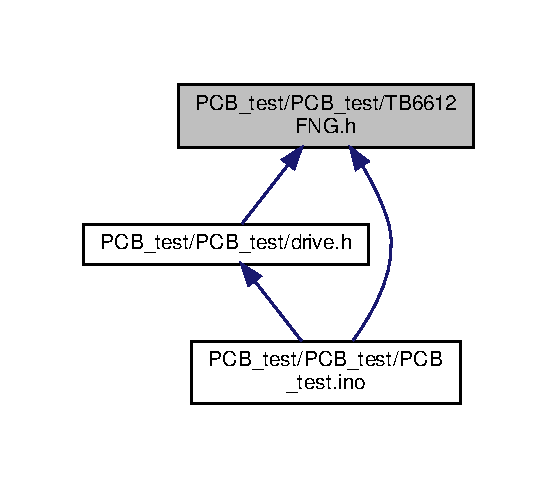
\includegraphics[width=268pt]{TB6612FNG_8h__dep__incl}
\end{center}
\end{figure}
\subsection*{Classes}
\begin{DoxyCompactItemize}
\item 
class \hyperlink{classMotorDriver}{Motor\+Driver}
\end{DoxyCompactItemize}
\subsection*{Variables}
\begin{DoxyCompactItemize}
\item 
const int \hyperlink{TB6612FNG_8h_a059bd507e81f5c1acf31887a06c61abd}{Rdir} = 4
\item 
\mbox{\Hypertarget{TB6612FNG_8h_af31057357531366da095242d79844028}\label{TB6612FNG_8h_af31057357531366da095242d79844028}} 
const int {\bfseries pwmR} = 6
\item 
\mbox{\Hypertarget{TB6612FNG_8h_ab4b58100911d5e2635258d949826ed2a}\label{TB6612FNG_8h_ab4b58100911d5e2635258d949826ed2a}} 
const int {\bfseries Ldir} = 9
\item 
\mbox{\Hypertarget{TB6612FNG_8h_a1fbf61284e18275b946866831c7efb94}\label{TB6612FNG_8h_a1fbf61284e18275b946866831c7efb94}} 
const int {\bfseries pwmL} = 5
\end{DoxyCompactItemize}


\subsection{Detailed Description}
Contains a low-\/level control interface for the motor driver chip. 



\subsection{Variable Documentation}
\mbox{\Hypertarget{TB6612FNG_8h_a059bd507e81f5c1acf31887a06c61abd}\label{TB6612FNG_8h_a059bd507e81f5c1acf31887a06c61abd}} 
\index{T\+B6612\+F\+N\+G.\+h@{T\+B6612\+F\+N\+G.\+h}!Rdir@{Rdir}}
\index{Rdir@{Rdir}!T\+B6612\+F\+N\+G.\+h@{T\+B6612\+F\+N\+G.\+h}}
\subsubsection{\texorpdfstring{Rdir}{Rdir}}
{\footnotesize\ttfamily const int Rdir = 4}

A\+Tmega328P, pwm works on pins 3, 5, 6, 9, 10, and 11 at 490/980\+Hz 
\hypertarget{util_8h}{}\section{P\+C\+B\+\_\+test/\+P\+C\+B\+\_\+test/util.h File Reference}
\label{util_8h}\index{P\+C\+B\+\_\+test/\+P\+C\+B\+\_\+test/util.\+h@{P\+C\+B\+\_\+test/\+P\+C\+B\+\_\+test/util.\+h}}


Contains a variety of miscellaneous math functions to allow for cleaner code.  


This graph shows which files directly or indirectly include this file\+:
\nopagebreak
\begin{figure}[H]
\begin{center}
\leavevmode
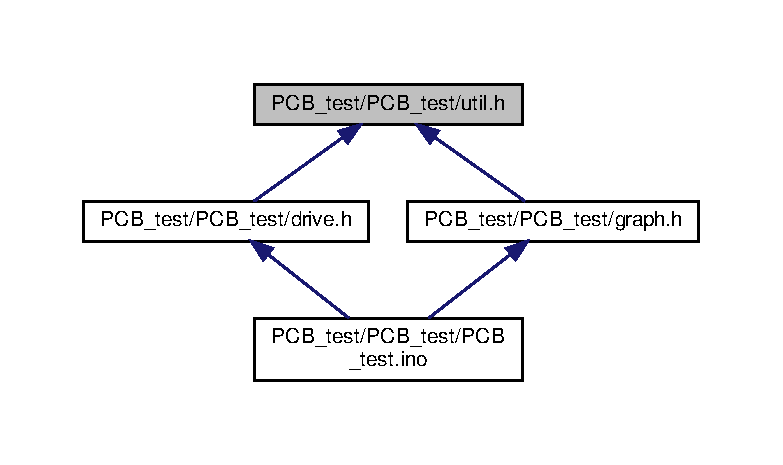
\includegraphics[width=350pt]{util_8h__dep__incl}
\end{center}
\end{figure}
\subsection*{Enumerations}
\begin{DoxyCompactItemize}
\item 
enum \hyperlink{util_8h_a92e22a126ad6bf9d255b517e70d083f6}{Direction} \+: byte \{ {\bfseries East} = (1 $<$$<$ 0), 
{\bfseries North} = (1 $<$$<$ 1), 
{\bfseries West} = (1 $<$$<$ 2), 
{\bfseries South} = (1 $<$$<$ 3)
 \}\begin{DoxyCompactList}\small\item\em Represents all directions in the maze. \end{DoxyCompactList}
\end{DoxyCompactItemize}
\subsection*{Functions}
\begin{DoxyCompactItemize}
\item 
\mbox{\Hypertarget{util_8h_ab3bf9f71e060eb5fe4c94a7c13eacc5a}\label{util_8h_ab3bf9f71e060eb5fe4c94a7c13eacc5a}} 
{\footnotesize template$<$typename T $>$ }\\T \hyperlink{util_8h_ab3bf9f71e060eb5fe4c94a7c13eacc5a}{signum} (const T \&value)
\begin{DoxyCompactList}\small\item\em A type-\/independent way to get the sign of a number. Returns -\/1, 0, or 1. \end{DoxyCompactList}\item 
\mbox{\Hypertarget{util_8h_af27cab9fc0fccc46073d5a597f38bf44}\label{util_8h_af27cab9fc0fccc46073d5a597f38bf44}} 
double \hyperlink{util_8h_af27cab9fc0fccc46073d5a597f38bf44}{accel\+Ramp} (double start, double target, double current)
\begin{DoxyCompactList}\small\item\em Returns a value between \mbox{[}0.\+0, 1.\+0\mbox{]}, based on how far between \textquotesingle{}start\textquotesingle{} and \textquotesingle{}target\textquotesingle{} the input \textquotesingle{}current\textquotesingle{} is. \end{DoxyCompactList}\item 
\mbox{\Hypertarget{util_8h_af40a993bf4371ac776eed7ce1ad3ab58}\label{util_8h_af40a993bf4371ac776eed7ce1ad3ab58}} 
double \hyperlink{util_8h_af40a993bf4371ac776eed7ce1ad3ab58}{decel\+Ramp} (double start, double target, double current)
\begin{DoxyCompactList}\small\item\em Like accel\+Ramp, but reversed (i.\+e. starts at 1.\+0 and decreases to 0.\+0). \end{DoxyCompactList}\item 
\mbox{\Hypertarget{util_8h_a61a31038d989bdef2da1d66b040f3912}\label{util_8h_a61a31038d989bdef2da1d66b040f3912}} 
double \hyperlink{util_8h_a61a31038d989bdef2da1d66b040f3912}{both\+Ramp} (double start, double target, double current)
\begin{DoxyCompactList}\small\item\em Combines accel\+Ramp and decel\+Ramp, switching from one to the other halfway between start and target. \end{DoxyCompactList}\end{DoxyCompactItemize}


\subsection{Detailed Description}
Contains a variety of miscellaneous math functions to allow for cleaner code. 



\subsection{Enumeration Type Documentation}
\mbox{\Hypertarget{util_8h_a92e22a126ad6bf9d255b517e70d083f6}\label{util_8h_a92e22a126ad6bf9d255b517e70d083f6}} 
\index{util.\+h@{util.\+h}!Direction@{Direction}}
\index{Direction@{Direction}!util.\+h@{util.\+h}}
\subsubsection{\texorpdfstring{Direction}{Direction}}
{\footnotesize\ttfamily enum \hyperlink{util_8h_a92e22a126ad6bf9d255b517e70d083f6}{Direction} \+: byte}



Represents all directions in the maze. 

These directions do N\+OT actually correspond to real cardinal directions. They are all relative to the robot\textquotesingle{}s starting position, which is in the South-\/\+Western corner, facing East. 
%--- End generated contents ---

% Index
\backmatter
\newpage
\phantomsection
\clearemptydoublepage
\addcontentsline{toc}{chapter}{Index}
\printindex

\end{document}
